\documentclass{standalone}

\usepackage{tikz}
\usetikzlibrary{calc}

\def\tikzscale{5}

\begin{document}

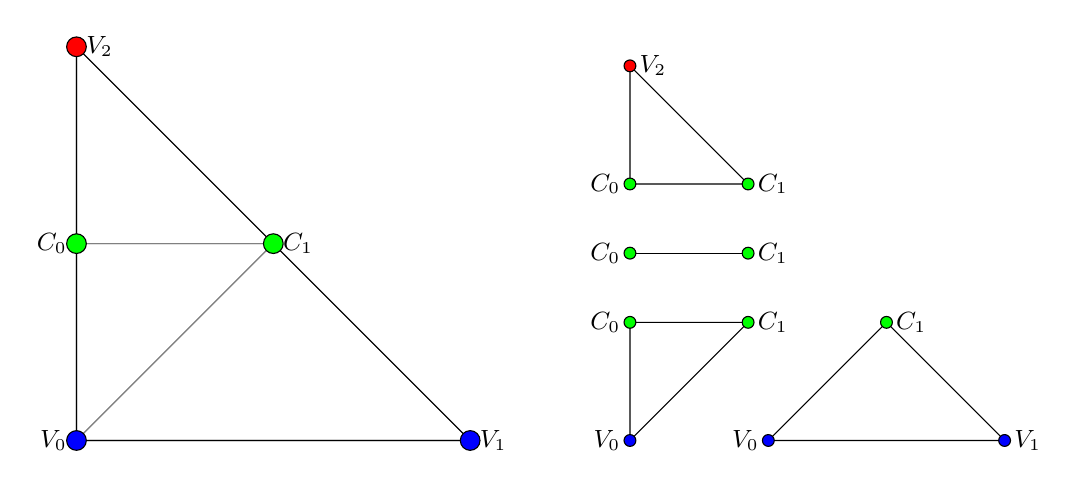
\begin{tikzpicture}[scale=\tikzscale]

  \def\Rad{0.25mm}


  \tikzstyle{every node}=[font=\small]

  \newcommand*{\DrawTri}[4]{%
    \draw[#1] (#2) -- (#3) -- (#4) -- cycle;
  }

  %% The original situation
  \begin{scope}[xshift=0,yshift=0]

    % corner points of main TET
    \coordinate (0) at (0, 0);
    \coordinate (1) at (1, 0);
    \coordinate (2) at (0, 1);

    % intersection points
    \coordinate (c0) at  ($0.5*(0)+0.5*(2)$);
    \coordinate (c1) at  ($0.5*(1)+0.5*(2)$);

    \DrawTri{gray}{c0}{c1}{2}
    \DrawTri{gray}{0}{c1}{c0}
    \DrawTri{gray}{0}{c1}{1}

    \DrawTri{black}{0}{1}{2}

    % vertices
    \draw[fill=blue] (0) circle (\Rad) node[left ]{$V_0$};
    \draw[fill=blue] (1) circle (\Rad) node[right]{$V_1$};
    \draw[fill=red ] (2) circle (\Rad) node[right]{$V_2$};

    % cut points
    \draw[fill=green] (c0) circle (\Rad) node[left ]{$C_0$};
    \draw[fill=green] (c1) circle (\Rad) node[right]{$C_1$};

  \end{scope}


  %% The top triangle
  \begin{scope}[xshift=40,yshift=10,scale=0.6]

    % corner points of main TET
    \coordinate (0) at (0, 0);
    \coordinate (1) at (1, 0);
    \coordinate (2) at (0, 1);

    % intersection points
    \coordinate (c0) at  ($0.5*(0)+0.5*(2)$);
    \coordinate (c1) at  ($0.5*(1)+0.5*(2)$);

    \DrawTri{black}{c0}{c1}{2}
    %%\DrawTri{black}{0}{c1}{c0}
    %%\DrawTri{black}{0}{c1}{1}

    %\DrawTri{black}{0}{1}{2}

    % vertices
    %%\draw[fill=blue] (0) circle (\Rad) node[left ]{$V_0$};
    %%\draw[fill=blue] (1) circle (\Rad) node[right]{$V_1$};
    \draw[fill=red ] (2) circle (\Rad) node[right]{$V_2$};

    % cut points
    \draw[fill=green] (c0) circle (\Rad) node[left ]{$C_0$};
    \draw[fill=green] (c1) circle (\Rad) node[right]{$C_1$};

  \end{scope}

  %% The surface
  \begin{scope}[xshift=40,yshift=5,scale=0.6]

    % corner points of main TET
    \coordinate (0) at (0, 0);
    \coordinate (1) at (1, 0);
    \coordinate (2) at (0, 1);

    % intersection points
    \coordinate (c0) at  ($0.5*(0)+0.5*(2)$);
    \coordinate (c1) at  ($0.5*(1)+0.5*(2)$);

    \draw[black] (c0) -- (c1);

    %%\DrawTri{black}{c0}{c1}{2}
    %%\DrawTri{black}{0}{c1}{c0}
    %%\DrawTri{black}{0}{c1}{1}

    %\DrawTri{black}{0}{1}{2}

    % vertices
    %%\draw[fill=blue] (0) circle (\Rad) node[left ]{$V_0$};
    %%\draw[fill=blue] (1) circle (\Rad) node[right]{$V_1$};
    %%\draw[fill=red ] (2) circle (\Rad) node[right]{$V_2$};

    % cut points
    \draw[fill=green] (c0) circle (\Rad) node[left ]{$C_0$};
    \draw[fill=green] (c1) circle (\Rad) node[right]{$C_1$};

  \end{scope}

  %% First bottom triangle
  \begin{scope}[xshift=40,yshift=0,scale=0.6]

    % corner points of main TET
    \coordinate (0) at (0, 0);
    \coordinate (1) at (1, 0);
    \coordinate (2) at (0, 1);

    % intersection points
    \coordinate (c0) at  ($0.5*(0)+0.5*(2)$);
    \coordinate (c1) at  ($0.5*(1)+0.5*(2)$);

    %%\DrawTri{black}{c0}{c1}{2}
    \DrawTri{black}{0}{c1}{c0}
    %%\DrawTri{black}{0}{c1}{1}

    %\DrawTri{black}{0}{1}{2}

    % vertices
    \draw[fill=blue] (0) circle (\Rad) node[left ]{$V_0$};
    %%\draw[fill=blue] (1) circle (\Rad) node[right]{$V_1$};
    %%\draw[fill=red ] (2) circle (\Rad) node[right]{$V_2$};

    % cut points
    \draw[fill=green] (c0) circle (\Rad) node[left ]{$C_0$};
    \draw[fill=green] (c1) circle (\Rad) node[right]{$C_1$};

  \end{scope}

  %% Second bottom triangle
  \begin{scope}[xshift=50,yshift=0,scale=0.6]

    % corner points of main TET
    \coordinate (0) at (0, 0);
    \coordinate (1) at (1, 0);
    \coordinate (2) at (0, 1);

    % intersection points
    \coordinate (c0) at  ($0.5*(0)+0.5*(2)$);
    \coordinate (c1) at  ($0.5*(1)+0.5*(2)$);

    %%\DrawTri{black}{c0}{c1}{2}
    %%\DrawTri{black}{0}{c1}{c0}
    \DrawTri{black}{0}{c1}{1}

    %\DrawTri{black}{0}{1}{2}

    % vertices
    \draw[fill=blue] (0) circle (\Rad) node[left ]{$V_0$};
    \draw[fill=blue] (1) circle (\Rad) node[right]{$V_1$};
    %%\draw[fill=red ] (2) circle (\Rad) node[right]{$V_2$};

    % cut points
    %\draw[fill=green] (c0) circle (\Rad) node[left ]{$C_0$};
    \draw[fill=green] (c1) circle (\Rad) node[right]{$C_1$};

  \end{scope}

\end{tikzpicture}
\end{document}

%%% Local Variables: 
%%% mode: latex
%%% TeX-master: t
%%% End: 
